\documentclass[a4paper]{jpconf}
\usepackage{graphicx}
\begin{document}
\title{The CMS DBS Query Language}

\author{Anzar Afaq, Vijay Sekhri, Yuyi Guo, Lee Lueking}
\address{Fermilab, Batavia, Illinois, USA}

%\author{Valentin Kuznetsov}
\author{Valentin Kuznetsov, Daniel Riley}
\address{Cornell University, Ithaca, New York, USA}

\begin{abstract}
The CMS experiment has implemented a flexible and 
powerful system enabling users to find data within 
the CMS physics data catalog. The Dataset Bookkeeping 
Service (DBS) comprises a database and the services 
used to store and access metadata related to CMS physics 
data.  To this, we have added a generalized query system
in addition to the existing web and programmatic interfaces to the DBS.
This query system is based on a query language that hides the 
complexity of the underlying database structure by discovering the join conditions between
database tables. This provides 
a way of query the system that is simple and straightforward for 
CMS data managers and physicists to use without requiring knowledge of the database
tables or keys. The DBS Query Language 
uses the ANTLR tool to build the input query parser and tokenizer, 
followed by a query builder that uses a graph representation of the 
DBS schema to construct the SQL query sent to underlying database. 
We will describe the design of the query system, provide 
details of the language components
and overview of how this component fits into the overall data 
discovery system architecture.
%We will also provide an 
%overview of how this component fits into the overall data 
%discovery system architecture, as well as providing access to other information sources
%such as the independent Data Quality and Luminosity databases.
\end{abstract}

\section{Introduction}

In anticipation of collecting data at the Large Hadron Collider (LHC),
the Compact Muon Solenoid (CMS) experiment has
developed a suite of sophisticated tools
to collect and record the metadata associated with the experimental data. At
LHC startup, the CMS experiment expects to collect a few
PB of data each year, which will be distributed to sites
around the world where physicists will explore the fundamental
interactions of our Universe. In a globally distributed system handling enormous volumes of data,
fast, efficient data look-up is a significant
challenge and also an essential ingredient for successful
analysis of the data. In the CMS data management system, the Data Bookkeeping
System\cite{DBS} is the authoritative record of
the data available for physics analysis. It collects
information from a broad variety of workflow tools used by CMS production teams, physics groups and individual physicists, allowing
CMS researchers to easily find the data relevant to their analyses.

\section{Searching for the tool}

Today there are two major technologies providing search capabilities
for end-users: relational Database Management Systems (DBMS), and Information Retrieval (IR) systems.
Each of these has its own strength and weaknesses, which
are outlined in table \ref{IR_DBMS}.

\begin{table*}[hbt]
\centering
\begin{tabular}{ll}\hline
\hline

IR & DBMS \\
\hline
Imprecise semantics & Precise semantics \\
Keyword search & SQL \\
Unstructured data & Structured data \\
Read-mostly, occasional updates & Frequent updates \\
Partial results (top N) & Complete results \\
\hline
\hline
\end{tabular}
\caption{Comparison of IR and DBMS characteristics}
\label{IR_DBMS}
\end{table*}

While these different kinds of systems are designed to address different problem domains,
in practice a blend of characteristics is often desirable. In High Energy Physics (HEP),
such merging of features is desirable in the LHC era to allow relatively unstructured
access to large volumes of structured data and metadata.

In HEP the experimental data are usually stored in many discrete files
residing on disk or tape, with the associated meta-data are stored in relational databases.
Physicists, however, are generally more comfortable with IR tools such as web search
engines, so the ideal interface to the metadata for physicists would combine the
relatively unstructured queries of IR tools with the precision semantics of DBMS query
languages.  In order to support such an interface, keywords provided by the physicist
({\it e.g., Higgs}) must be mapped to a search on a specific set of
table columns in the underlying database schema and translated into an appropriate query.
In addition, our users want
to search for data satisfying specific sets of conditions, selecting only those
data satisfying the criteria. For example, 
{\it I want a sample of Higgs candidate events processed with software release
1.2.3 in the range of runs between 100 and 200}.  Such requests are
easier to formulate using the precise semantics of DBMS query languages.
These use cases were reviewed by us\cite{DBS07}
during the development of the CMS Data Discovery tool. We explored
a variety of user interfaces and methods to address this mixture of requirements, resulting
in a domain-specific DBS Query Language (QL) that uses a mixture
of both approaches, IR and DBMS, combining the precise
semantics of a DBMS query language with the flexibility of
IR system keyword searches.

\section{From SQL to QL}

The quantity of information stored in the CMS DBS system already
presents challenges for physicists and data managers searching for
data sets with specific characteristics.
Several user interfaces were proposed to address this issue, including
structured top-down approaches where users pick characteristics
from lists of known entities, such as
trigger line, dataset name, etc.
While this approach, implemented using drop-down menus,
was very intuitive to learn,
it rapidly encountered scaling limits as the number of entries to in the drop-down menus
became unwieldy.
Management of such large lists in the browser interface presents significant challenges,
negating the conceptual simplicity of the interface. This led us to consider alternate
approaches, eventually leading to the design of
DBS QL as the primary user interface for finding data in the DBS.

The DBS QL syntax was intentionally kept very close to SQL.  With some minor amendments, this syntax naturally
maps into the user mental model and was easily adopted by the CMS
community. After several iterations of user testing, we adopted the following syntax:
\[
find\,\,\,
key_1,\, key_2,\, ...\,\,\, where\,\,\,
\langle key\rangle\, 
\langle op\rangle\, 
\langle value\rangle \,\,\, and|or ...
\label{QL_syntax}
\]
Here $find, where, and, or$ are reserved keywords
adapted from SQL syntax\footnote{Except for the {\it find} special
keyword we used all SQL keywords, e. g. {\it between, in}, etc.}
The keys for both selection and condition are defined
in DBS QL based on standard terminology used by physicists, {\it e.g.,} dataset, file, run. 
These keywords are mapped into internal database table columns or entire tables,
structured as entities and their attributes. For example,
the {\it file} keyword can map directly to the file name attribute, or it can represent the file
entity which maps to the file table. The file table
contains more information about files, including the size, creation time,
type etc. These can be accessed as attributes of the file entity, {\it e.g.,}
{\it file.size, file.createdate, file.type}. Some attributes
are present for all QL keys, {\it e.g.,} {\it createdate, createby}, {\it etc.},
while other attributes are unique to certain entities, {\it e.g.,} {\it release.family}.

To accommodate a variety of search criteria, DBS QL supports
the usual set of boolean operators, including $>, >=, <, <=, =, like$, {\it etc.};
details can be found in the $\langle op\rangle$ section of \ref{QL_syntax}.
Since a DBS QL query is mapped directly to SQL, our limitations query expressivity
are derived from SQL.  Complex queries can be expressed using
brackets and combinations of constraints.

Figure \ref{Grammar} represents a simplified view of the grammar
that defines the syntax of the DBS QL.
\begin{figure}[htb]
\centering
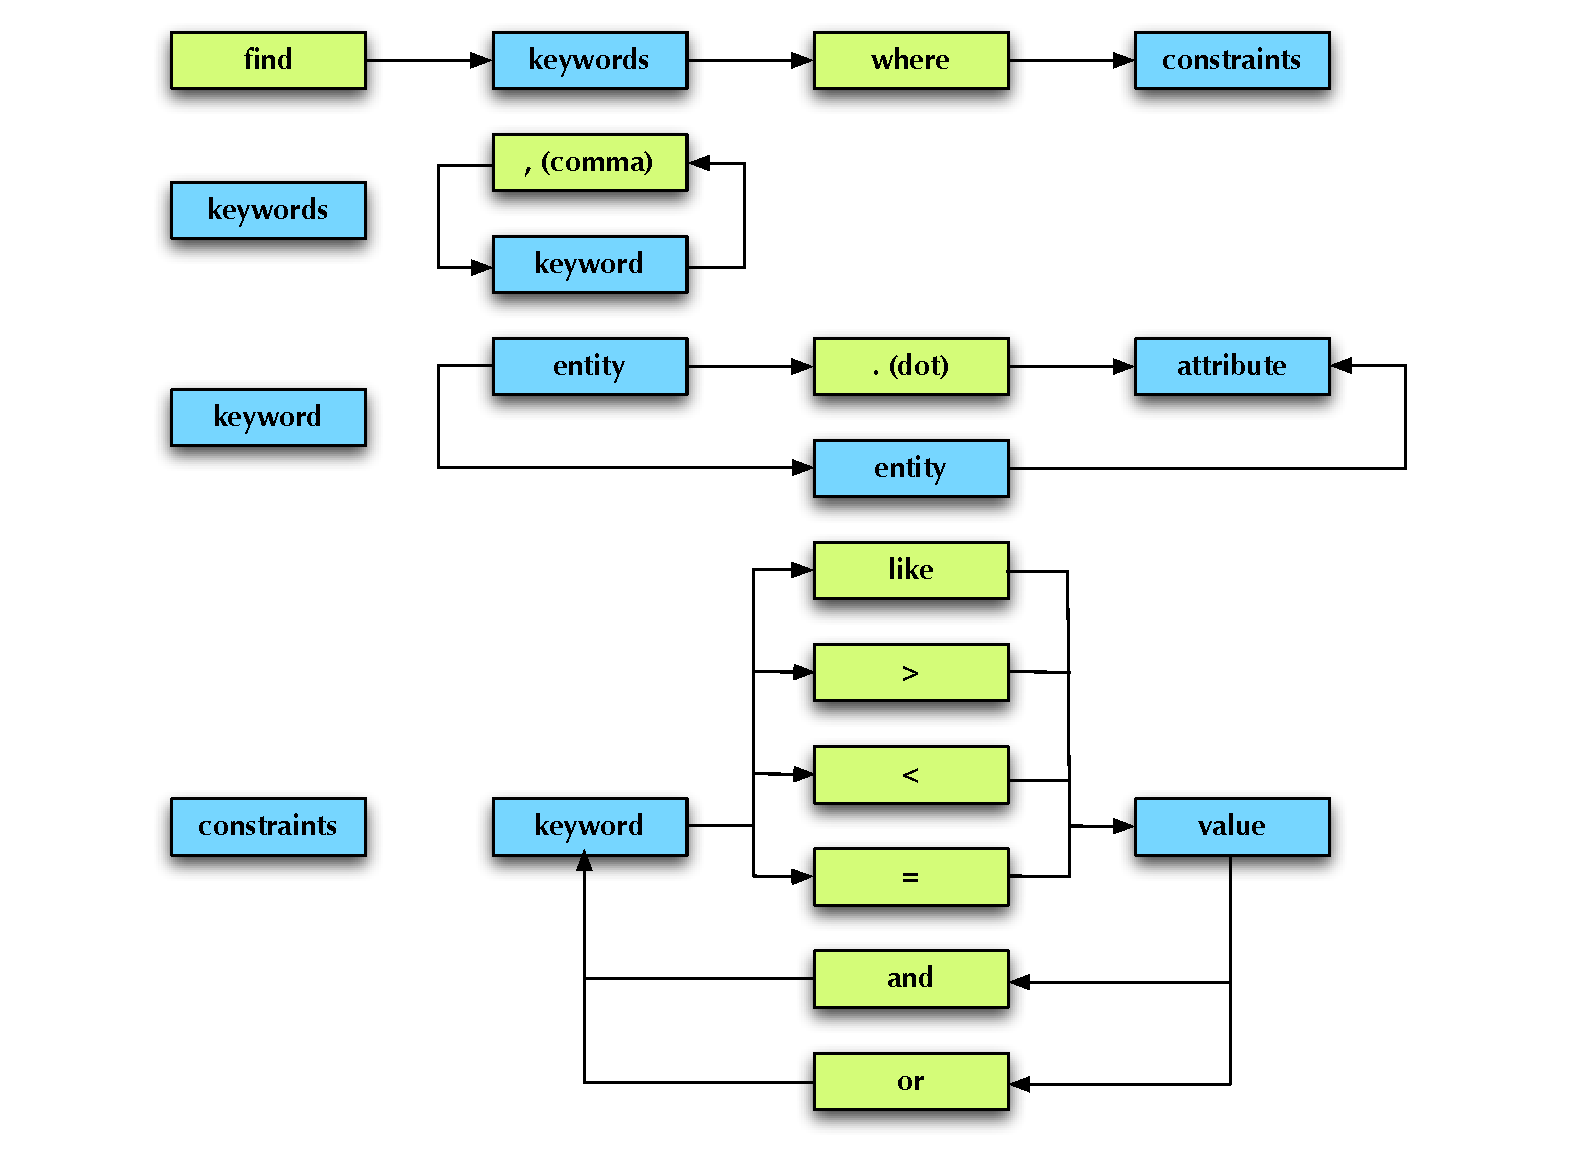
\includegraphics[width=150mm]{DBSSql_grammar.pdf}
\caption{
DBS QL grammar.
}
\label{Grammar}
\end{figure}
In this diagram the entities (keywords) represent logical tables. 
Each entity has a set of additional attributes (columns). 
The grammar allows any combination of entity and
attribute, however not every attribute
is appropriate for every entity.  Incorrect
combinations are detected by the Query Builder at query construction time,
and appropriate diagnostics are provided to the end-user with the
precise position of the error.  Aggregation functions, such
as sum and count, are also supported.

Note that the DBS QL grammar does not
include any explicit {\it join} operation.
This syntax gives us great flexibility to construct
arbitrary queries against the DBS using published DBS QL keys.
To translate these queries into standard SQL, we define an external mapping between
tables and graph nodes using
Dijkstra’s shortest path algorithm to find the join conditions
implied by the user's query.  This is discussed in detail in the next section.

\section{DBS QL architecture}

The DBS design uses the well-known 3-tier architecture. The server
code is implemented using Java Servlets in a Tomcat container.
The details have been discussed elsewhere\cite{DBS} and will not
be covered here. 

DBS QL was first prototyped in Python and subsequently re-implemented
in Java using the ANTRL parser generator. The architecture is shown in Fig. \ref{DBS_QL}.
\begin{figure}[htb]
\centering
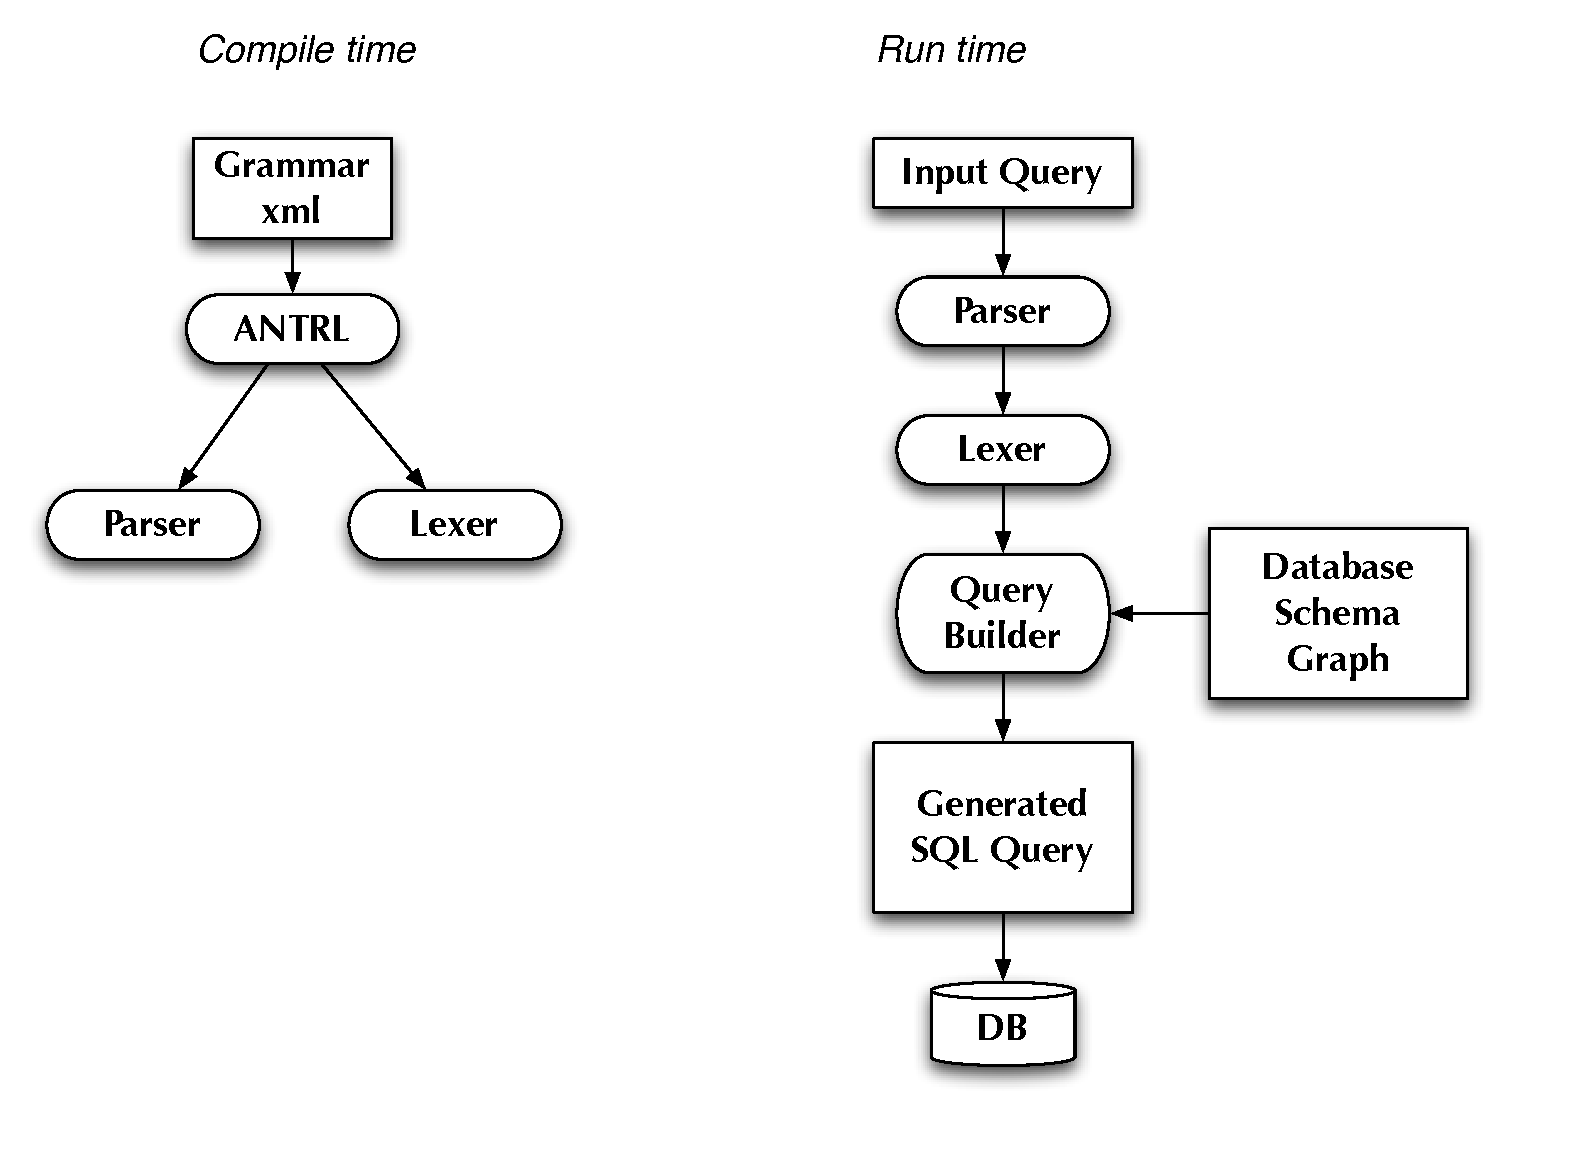
\includegraphics[width=100mm]{DBS_QL_architecture.pdf}
\caption{DBS QL architecture.}
\label{DBS_QL}
\end{figure}
At compile time, ANTLR\cite{ANTLR} processes the DBS QL grammar description to generate
the language parser and lexer.  When a query is processed, the parser and lexer tokenize
the DBS QL query, which is then translated into an SQL query by the query builder.
One drawback of this scheme is that entity and attribute names are part of the DBS QL
grammar, so changes to the database schema may require corresponding changes to the
language grammar.

%Regardless of UI (web or command-line), the user query was 
%passed to the server where it was interpreted by a lexer and a parser.
%Then the Query Builder generates a valid SQL query suitable for
%execution at DB back-end.\footnote{We officially supported ORACLE and
%MySQL back-ends.} 
%The ANTLR tool was used an external grammar file which defined 
%the syntax and semantics of DBS QL. It generated the parser and lexer 
%code for compile time. Therefore a new addition to QL, such as key,
%attribute and/or support for boolean expression, had a drawback of
%regenerating the parser and lexer code and its redeployment on a server.
 
In order to discover the joins implicit in DBS QL queries,
the database schema is represented as a weighted
directed graph with nodes mapped to tables and edges 
representing relationships between tables\cite{GraphTool}.
The Query Builder
uses Dijkstra’s shortest path algorithm to determine the least-weight 
path from one table to another and resolve multi-path ambiguities.
The chosen path is used to construct the table joins in the final SQL query. 
For example, figure \ref{ShortestPath} shows database tables 
T1 through T4 where edges between the tables represents the 
relationships between the tables.

\begin{figure}[htb]
\centering
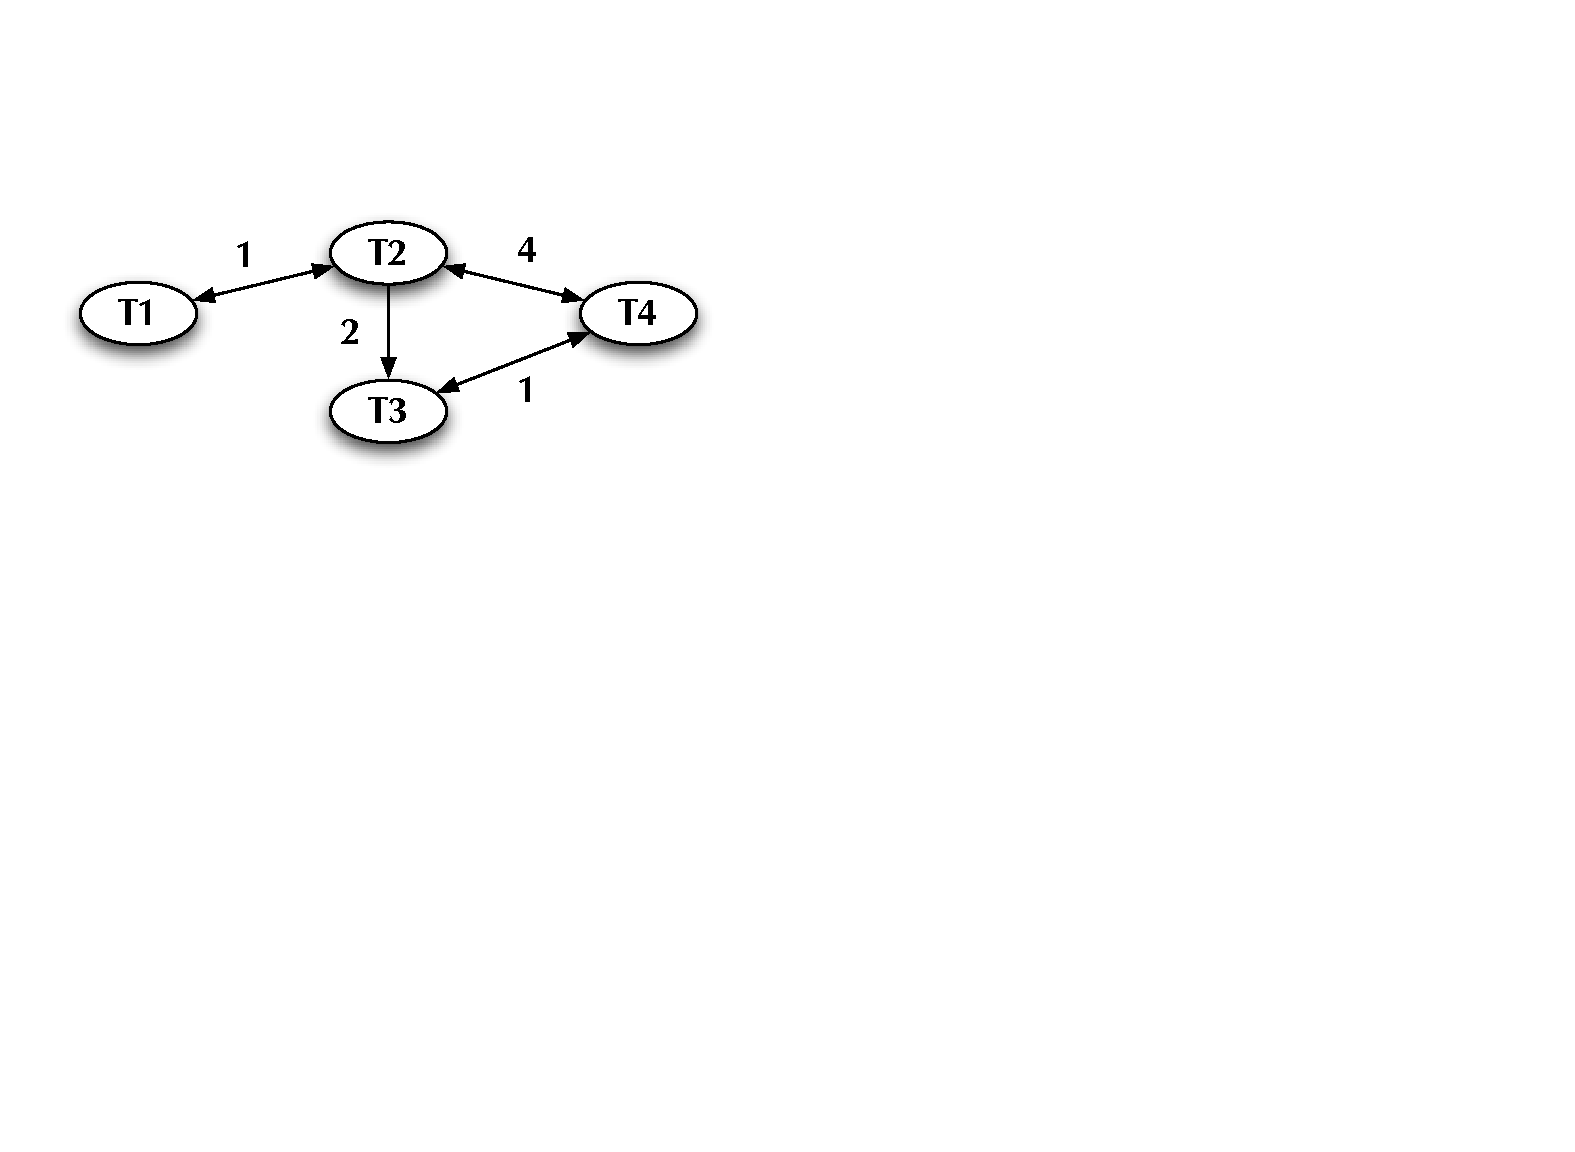
\includegraphics[width=80mm]{DBSSql_shortestpath.pdf}
\caption{A graph illustrating different paths between tables. The
numbers are weights assigned to each possible table join, from which the least-cost path
is computed. For example, the shortest path from table T1 to T4 is 
T1 $\rightarrow$ T2 $\rightarrow$ T3 $\rightarrow$ T4 with total weight 
of 4.  The shortest path from table T4 to T1 is 
T4 $\rightarrow$ T2 $\rightarrow$ T1, with total weight of 5, because the path
from T3 to T2 is prohibited (infinite weight).
}
\label{ShortestPath}
\end{figure}
Where ambiguities arise between two or more paths
with identical cost, the edge weights are manually adjusted to remove the
ambiguity, guided by concrete use cases. 
% Such resolution was done in external schema graph file.

Since DBS QL hides all explicit relationships between tables and does not
expose the actual table names, users may
specify any combination of entities and attributes in their queries.\footnote{
A time limit is applied to the evaluation of the generated SQL queries
in order to avoid long running queries from loose query conditions.}
These are mapped to table, columns, keys and joins according to
shortest connecting path found by the Query Builder in the schema graph.
All necessary joins, keys and intermediate tables are found as part of the
graph traversal.
In the aforementioned example \ref{ShortestPath},
if the user specified
$$find\,\, key_1, key_4\,\, where\,\, ...$$
where $key_1, key_4$ map to T1 table and T4 tables respectively,
the Query Builder determines
the shortest path 
T1$\rightarrow$T2$\rightarrow$T3$\rightarrow$T4 
and adds the intermediate tables 
and join conditions to form the final SQL query. 

This process can be illustrated via an example translation of a
DBS QL query into SQL.  A user wants the answer to the following
question: {\it I want to find the number of files and their total
size for all files which belong to a dataset where the dataset name begins with
the string ``Online''
and the run number is less then 224. In addition I want to restrict the query
to files with size less then 10}. This question can be
expressed in DBS QL as simply as
%find file.count, file.size where 
\begin{verbatim}
find count(file), sum(file.size) where 
     file.size > 10 and run < 224 and dataset = Online*
\end{verbatim}
One measure of how well our query language fits the mental model of our users is
how easily and intuitively the informal query translates into DBS QL.
From this, the Query Builder constructs the following SQL expression:
\begin{verbatim}
SELECT COUNT(DISTINCT COUNT_SUB_Files) AS COUNT_Files, 
    Files_FileSize AS Files_FileSize  
    FROM (SELECT DISTINCT Files.LogicalFileName AS COUNT_SUB_Files
         ,Files.FileSize AS Files_FileSize
            FROM Files
            JOIN FileRunLumi ON FileRunLumi.Fileid = Files.ID
            JOIN Runs ON Runs.ID = FileRunLumi.Run
            WHERE Files.FileSize > :p0 
                  AND Runs.RunNumber < :p1
                  AND Files.Block IN 
                  (SELECT Block.ID FROM Block 
                   WHERE upper(Block.Path) LIKE upper(:p2) )
             AND FileRunLumi.Fileid = Files.ID
             AND FileRunLumi.Run = Runs.ID
         ) sumtable GROUP BY Files_FileSize
<p0>10</p0> <p1>224</p1> <p2>Online%</p2>
\end{verbatim}
(where p0, p1 and p2 specify Oracle variable bindings\footnote{We officially support Oracle and
MySQL back-ends.}).
By default we use JOIN relationships between all tables where associative
constrains exist, either via unique key or foreign key relationships,
but in some cases ``LEFT OUTER JOIN'' is more appropriate.
Aggregation is done via sub-queries.

The ordering may also be specified in DBS QL via {\it order by}
expressions, {\it e.g.,}
\begin{verbatim}
find dataset where run > 100 order by run desc
\end{verbatim}
In this example, the relationship between dataset and run
must be discovered to allow proper ordering.
We also support a variety of time-stamp formats, {\it e.g.,}
\begin{verbatim}
find file where file.createdate = 2007-04-20 11:27:21 CDT 
     or file.moddate > 2008 or run = 234
\end{verbatim}
This is a very convenient feature for an international collaboration.
All such rules are easy to implement and adjust via the ANTLR parser grammar.

In some cases auto-generated queries have poor efficiency, especially
when multiple selection keys and conditions are specified. To address this
issue we are evaluating procedures for replacing specific auto-generated queries with
hand-written ones.  For simple look-ups of a single entity, e.g. {\it find dataset}
or {\it find run}, we use DB views to aggregate information
about the entity.  These views generate summary information using manually optimized queries
For example, for the query {\it find dataset},
we use a pre-defined summary view which finds the number of blocks and
files in the dataset, its total size, the number of events, and the integrated luminosity. 
This approach increases the usability of the interface and optimizes the underlying
query. Moreover, when new information about an entity is added,
we just update the underlying view, making the change transparent.

It is worth noting that DBS QL can be adopted to
any DB schema, using any standard SQL DB back-end and programming interface.
What DBS QL provides is additional mapping between your data model and
user interface by making a bridge between the user's mental model
and the relational model of your data. 
Changes in the model can be accommodated
transparently via new mappings the in DBS QL grammar.
% In fact,
%such changes where successfully done during different release cycles of
%DBS QL implementation.

Providing this mapping enables
users to make complex queries without detailed knowledge of
the underlying data model. 
In fact, as will be discussed in the
next section, we are currently exploring the possibility of
expanding DBS QL to other CMS data services, seamlessly combining them
into a single aggregated service that can be queried through a single interface.

%Finally, DBS QL completes the overall picture of data provenance in CMS data model.
%The DBS QL queries together with meta-data information stored in files represented
%a full stack of provenance information. Also, they can be used
%as an input for further analysis of commonly used queries, providing a way for
%optimization DBS service via pre-fetching mechanism.

\section{DBS QL integration with other CMS services}

DBS QL has rapidly become the interface of choice to search for
CMS data. Due to the simple web interface provided by the CMS
Data Discovery\cite{DD} system and its integration with DBS QL,
users are able to find their data quickly and
efficiently. Over time the Data Discovery UI has
changed several times, from the original menu-driven approach using
a direct connection to the DB to the current DBS QL presentation layer
using a stateless connection to any DBS instance deployed
within CMS. Our users have started adopting DBS QL for their
own applications, performing monitoring of their
site usage, customizing views for data-centers
and developing easy to use new services, such as
FileMover\cite{FileMover}. To demonstrate the simplicity and
flexibility of the DBS QL interface to the underlying services,
here is a simple, but realistic,
code snippet in Python to query the run summary information
for a specified dataset
\begin{verbatim}
import urllib, urllib2

dbsurl = "http://host/DBSServlet"
query  = "find run, run.numevents, count(file) where dataset=/a/b/c"
params = {'apiversion':'DBS_2_0_6','api':'executeQuery', 'query': query} 
data=urllib2.urlopen(dbsurl,urllib.urlencode(params).read()
result = data.read()
\end{verbatim}
In addition to the Data Discovery web interface, the DBS also
provides a simple stand-alone command line tool
to search data from users in their
favorite environments. This tool was written
in Python, does not require any external dependencies, and can
be used on any OS used within CMS.

Moreover, the simplicity of DBS QL led us to explore a further
extension of the query language to other data-services deployed in CMS, under
the umbrella of our Data Aggregation Service (DAS). The DAS idea is
novel within CMS and still under development.
It allows users to place queries across multiple CMS data services,
such as the DBS, SiteDB, PhEDEx, Luminosity DB, etc.  Its syntax
is based on DBS QL, naturally
expanding the boundaries to other services, providing
end-users the ability to combine multiple services in simple, intuitive
queries. But instead of mapping DAS QL into a single
schema graph, we are exploring how to map it to a set of data-service APIs.

\section{Summary}
We have discussed a novel approach to searching CMS data,
based on a flexible,
intuitive and expandable query language using
semantics close to the mental model physicists use in their 
daily operations.
By hiding relationships and mapping well-known
keys and their attributes onto underlying data-service
schema, we achieve a simple yet scalable query language. Its 
has been widely adopted within CMS via the Data Discovery web interface and
in various workflow and analysis tools. Physicists
are able to quickly answer their questions about data by
specifying selection keys and providing set of conditions
in their query. We have demonstrated that this approach
can, in principle, be adopted to any SQL database schema and can be implemented
in any language.

\section{Acknowledgements}

This work was supported by the National Science Foundation and Department of Energy of the United States of America.

\section*{References}
\begin{thebibliography}{9}
\bibitem{DBS} A. Afaq, et. al. ``The CMS Dataset Bookkeeping Service'', CHEP 2007 
\bibitem{DBS07} A. Dolgert, V. Kuznetsov, C. Jones, D. Riley, 
``A multi-dimensional view on information retrieval of CMS data'', CHEP 2007
\bibitem{DD} https://cmsweb.cern.ch/dbs\_discovery
\bibitem{ANTLR} http://www.antlr.org
\bibitem{GraphTool} http://www.ics.uci.edu
\bibitem{FileMover} B. Bockelman, V. Kuznetsov ``CMS FileMover: one click data'', CHEP 2009

\end{thebibliography}

\end{document}


